
\medskip
O diagrama a seguir representa o Modelo Entidade–Relacionamento (DER) do sistema \textit{Nitrusleaf}, 
descrevendo a estrutura lógica do banco de dados. As entidades, seus atributos e os relacionamentos 
foram definidos conforme os requisitos do sistema, assegurando integridade e suporte às funcionalidades 
de operação e análise.

\medskip
A entidade \textbf{Usuários} centraliza as informações de acesso e cadastro 
(incluindo \textit{tipo\_pessoa}, foto, CPF/CNPJ e dados de contato/endereço). Ela se relaciona 
com \textbf{Propriedades} pelo relacionamento \textbf{Possui}: um usuário pode não possuir ou 
possuir várias propriedades (0:N) e cada propriedade pertence a um único usuário (1:1).
\medskip

As \textbf{Propriedades} armazenam dados cadastrais (logradouro, CEP, cidade) e contadores globais 
(\textit{talhoes\_registrados}, \textit{total\_pes}). Cada propriedade \textbf{contém} múltiplos 
\textbf{Talhões} (1:N) e também \textbf{contém} diversos \textbf{Alqueires} (1:N). Os \textbf{Talhões} 
registram metadados produtivos (espécie/fruta, \textit{total\_pes}, \textit{pes\_analisados}, 
\textit{pes\_diagnosticados}).
\medskip

Dentro de cada talhão são cadastrados os \textbf{Pés} (plantas individuais), em relacionamento 1:N 
(Talhão~$\rightarrow$~Pés). A entidade \textbf{Pés} guarda a situação atual e campos de diagnóstico 
(\textit{deficiencia\_cobre}, \textit{deficiencia\_manganes}, \textit{outros}, \textit{observacoes}).
\medskip

O histórico temporal de cada planta é mantido por \textbf{Historico\_pe}, ligado a \textbf{Pés} pelo 
relacionamento \textbf{Armazena}: um pé pode possuir muitos registros (descrição, \textit{data\_criacao}, 
situação) e cada registro referencia um único pé (e seu talhão no momento do evento).
\medskip

As avaliações visuais são registradas em \textbf{Fotos}. Pelo relacionamento \textbf{Analisado\_por}, 
um Pé pode ter muitas fotos (1:N) e cada Foto está vinculada a um único pé (URL, \textit{data\_tiragem}, 
\textit{resultado\_analise}).
\medskip

A partir das fotos, o sistema gera \textbf{Relatórios}. Cada Relatório é produzido a partir de uma 
única Foto e vincula-se a um único Pé, consolidando \textit{data da análise}, achados de deficiência 
(cobre, manganês, outros) e observações. O relacionamento \textbf{Tem\_relatorios} expressa que um pé 
pode possuir vários relatórios (1:N), e \textbf{Gera} indica a origem do relatório a partir de uma foto 
(uma foto pode originar relatórios reprocessados).
\medskip

\begin{figure}[H]
\centering
\caption{Diagrama Entidade–Relacionamento}
\label{fig:diagrama-der}
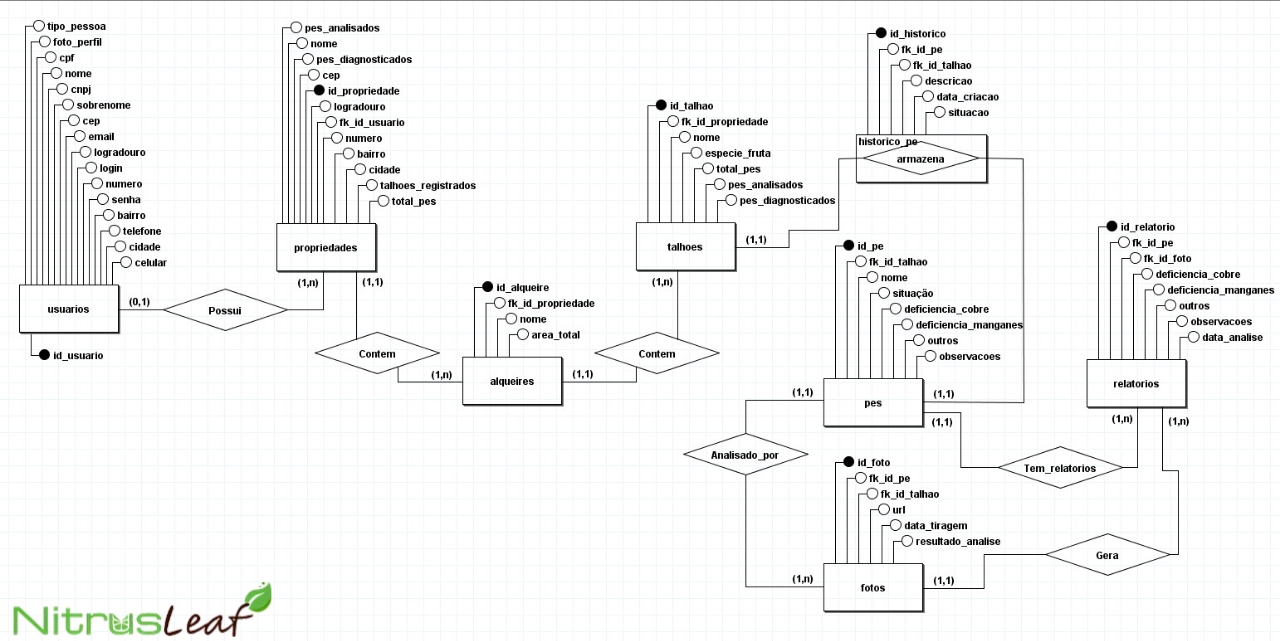
\includegraphics[width=0.9\textwidth]{Images/DiagramaDER.jpg}
\SourceOrNote{Equipe 21 -- Vitalliz (2025)}
\end{figure}

Esse modelo é fundamental para garantir a integridade dos dados e a correta
estruturação das informações no sistema.
\medskip